\documentclass[aspectratio=169, 10pt]{beamer}

% ==============================================================================
% Theme & Styling (Amrita Medical AI Blue Palette)
% ==============================================================================
\usetheme{Madrid}

\usepackage[utf8]{inputenc}
\usepackage{amsmath, amssymb, amsfonts}
\usepackage{booktabs}
\usepackage{tikz}
\usetikzlibrary{shapes, arrows.meta, positioning, calc, backgrounds, fit}
\usepackage{graphicx}
\usepackage{tabularx}
\usepackage{colortbl}
\usepackage{hyperref}

% Custom Professional High-Contrast Medical Blue Palette
\definecolor{AmritaBlue}{RGB}{14, 54, 97}       % Deep Navy / Amrita Blue
\definecolor{MedBlue}{RGB}{28, 92, 148}         % Primary Clinical Blue
\definecolor{LightBlue}{RGB}{236, 244, 252}     % Soft Clean Background
\definecolor{AccentCyan}{RGB}{0, 164, 214}      % Accent Cyan
\definecolor{DarkText}{RGB}{25, 30, 36}         % High-contrast body text
\definecolor{SuccessGreen}{RGB}{20, 125, 68}    % Metric Match Green
\definecolor{AlertRed}{RGB}{196, 40, 30}        % Alert Accent

% Color configuration
\setbeamercolor{normal text}{fg=DarkText, bg=white}
\setbeamercolor{structure}{fg=MedBlue}
\setbeamercolor{palette primary}{bg=AmritaBlue, fg=white}
\setbeamercolor{palette secondary}{bg=MedBlue, fg=white}
\setbeamercolor{palette tertiary}{bg=LightBlue, fg=AmritaBlue}

% Title and Frame Title Colors & Fonts (Pure high-contrast white on navy blue)
\setbeamercolor{title}{bg=AmritaBlue, fg=white}
\setbeamercolor{subtitle}{fg=AccentCyan}
\setbeamerfont{title}{series=\bfseries, size=\large}
\setbeamerfont{subtitle}{series=\mdseries, size=\small}

\setbeamercolor{frametitle}{bg=AmritaBlue, fg=white}
\setbeamerfont{frametitle}{series=\bfseries, size=\normalsize}

% Blocks styling
\setbeamercolor{block title}{bg=MedBlue, fg=white}
\setbeamercolor{block body}{bg=LightBlue, fg=DarkText}
\setbeamercolor{block title example}{bg=SuccessGreen, fg=white}
\setbeamercolor{block body example}{bg=LightBlue, fg=DarkText}
\setbeamercolor{block title alerted}{bg=AlertRed, fg=white}
\setbeamercolor{block body alerted}{bg=LightBlue, fg=DarkText}

\setbeamertemplate{navigation symbols}{}
\setbeamertemplate{blocks}[rounded][shadow=true]

% Clean Full-Width Frametitle Banner with Crisp White Text
\setbeamertemplate{frametitle}{%
  \nointerlineskip%
  \begin{beamercolorbox}[wd=\paperwidth,ht=3.2ex,dp=1.2ex,leftskip=0.8cm,rightskip=0.8cm]{frametitle}%
    \strut\textbf{\textcolor{white}{\insertframetitle}}\strut%
  \end{beamercolorbox}%
}

% Suppress duplicate top headline to maximize vertical slide area & alignment
\setbeamertemplate{headline}{}

% Professional Three-Segment Footline (Anonymous / Course-Centric)
\setbeamertemplate{footline}{%
  \leavevmode%
  \hbox{%
  \begin{beamercolorbox}[wd=.36\paperwidth,ht=2.5ex,dp=1.1ex,leftskip=0.5cm]{palette primary}%
    \usebeamerfont{author in head/foot}\textbf{Course 22AIE437: Medical Image Processing}
  \end{beamercolorbox}%
  \begin{beamercolorbox}[wd=.36\paperwidth,ht=2.5ex,dp=1.1ex,center]{palette secondary}%
    \usebeamerfont{title in head/foot}HAPPY Placenta Histology Replication
  \end{beamercolorbox}%
  \begin{beamercolorbox}[wd=.28\paperwidth,ht=2.5ex,dp=1.1ex,rightskip=0.5cm,right]{palette primary}%
    \usebeamerfont{date in head/foot}Academic Year 2026 \quad \insertframenumber{} / \inserttotalframenumber%
  \end{beamercolorbox}}%
  \vskip0pt%
}

% Title Information
\title[HAPPY Placenta Histology Replication \& Novelty]{HAPPY: Hierarchical Cellular-to-Tissue Phenotyping of Placenta Histology \& Attention-Enhanced Cell Classification}
\subtitle{Course 22AIE437: Medical Image Processing --- Final Project Presentation}

\author[Course 22AIE437]{
  \textbf{Student Roll Numbers:} \\
  \vspace{0.15cm}
  \textbf{CB.SC.U4AIE23258} \quad \textbf{CB.SC.U4AIE23249} \quad \textbf{CB.SC.U4AIE23253} \\
  \vspace{0.25cm}
  \textit{B.Tech Computer Science \& Engineering (Artificial Intelligence)}
}

\institute[Amrita Vishwa Vidyapeetham]{
  Amrita School of Artificial Intelligence \\
  Amrita Vishwa Vidyapeetham, Coimbatore
}

\date{Academic Year 2026}

% ==============================================================================
% Document Body
% ==============================================================================
\begin{document}

% ------------------------------------------------------------------------------
% Slide 1: Title Slide
% ------------------------------------------------------------------------------
\begin{frame}[plain]
  \titlepage
\end{frame}

% ------------------------------------------------------------------------------
% Slide 2: Problem & Motivation (Section 1: Introduction - Part 1)
% ------------------------------------------------------------------------------
\begin{frame}{Problem Formulation and Clinical Motivation}
\begin{columns}[onlytextwidth, t]
  \begin{column}{0.47\textwidth}
    \begin{block}{The Clinical Challenge: Placenta Histology}
      \parbox[t][4.9cm][t]{\linewidth}{
        \begin{itemize}\small
          \item The placenta is the vital temporary organ governing fetal oxygenation and nutrition; pathological lesions directly cause \textbf{preeclampsia, fetal growth restriction (FGR), and stillbirth}.
          \item Digitized Whole Slide Images (WSIs) span \textbf{billions of pixels} (gigapixel scale) with dense cellular heterogeneity.
          \item Manual slide reading by pathologists suffers from \textbf{high inter-observer variability} and specialist shortages.
        \end{itemize}
      }
    \end{block}
  \end{column}
  \hfill
  \begin{column}{0.47\textwidth}
    \begin{block}{Why Hierarchical AI is Required}
      \parbox[t][4.9cm][t]{\linewidth}{
        \begin{itemize}\small
          \item Patch-level CNNs ignore spatial tissue architecture and cell-to-cell signaling.
          \item Pathologists assess tissue via a \textbf{bottom-up hierarchy}:
            \begin{enumerate}\footnotesize
              \item Identify individual cell nuclei.
              \item Classify cell phenotypes (trophoblasts, stroma, endothelial).
              \item Group spatial clusters into villous tissue structures.
            \end{enumerate}
          \item We replicate and enhance \textbf{HAPPY} (\textit{Nature Comms} 2024), an end-to-end bottom-up phenotyping framework.
        \end{itemize}
      }
    \end{block}
  \end{column}
\end{columns}
\end{frame}

% ------------------------------------------------------------------------------
% Slide 3: Dataset, Objectives & Metrics (Section 1: Introduction - Part 2)
% ------------------------------------------------------------------------------
\begin{frame}{Dataset Characteristics and Evaluation Objectives}
\begin{columns}[onlytextwidth, t]
  \begin{column}{0.47\textwidth}
    \begin{block}{Multi-Center Histology Dataset (Zenodo)}
      \parbox[t][4.9cm][t]{\linewidth}{
        \begin{itemize}\small
          \item \textbf{Clinical Cohorts}: HMC, UOT, and NUH hospitals.
          \item \textbf{Stage 1 (Nuclei)}: 2,754 test nuclei across 38 held-out histological images.
          \item \textbf{Stage 2 (Cell Phenotypes)}: 18,946 cell patches ($224\times 224$); \textbf{2,743 held-out test cells} across 11 classes.
          \item \textbf{Stage 3 (Tissue Graphs)}: Whole slide graphs; \textbf{144,241 labeled test nodes} on official spatial split.
        \end{itemize}
      }
    \end{block}
  \end{column}
  \hfill
  \begin{column}{0.47\textwidth}
    \begin{block}{Tasks and Evaluation Metrics}
      \parbox[t][4.9cm][t]{\linewidth}{
        \begin{itemize}\small
          \item \textbf{Stage 1 Localisation (Detection)}:
            \begin{itemize}\footnotesize
              \item Object Precision, Recall, \textbf{F1-score} (IoU $\ge 0.5$).
            \end{itemize}
          \item \textbf{Stage 2 Cell Classification}:
            \begin{itemize}\footnotesize
              \item \textbf{Accuracy}, Top-2 Accuracy, Macro ROC-AUC (OvO).
            \end{itemize}
          \item \textbf{Stage 3 Tissue Classification (GNN)}:
            \begin{itemize}\footnotesize
              \item Node-level \textbf{Accuracy}, Top-2, Top-3, Macro ROC-AUC.
            \end{itemize}
        \end{itemize}
      }
    \end{block}
  \end{column}
\end{columns}
\end{frame}

% ------------------------------------------------------------------------------
% Slide 4: Base Paper Overview (Section 2: Base Paper - Part 1)
% ------------------------------------------------------------------------------
\begin{frame}{Base Paper Overview: HAPPY Framework}
\begin{block}{Base Paper Citation}
  \small
  \textbf{Title:} \textit{A hierarchical approach for whole slide histology phenotyping of the human placenta (HAPPY)} \\
  \textbf{Authors:} R. Vanea, G. H. Verghese, P. D. A. Higgins, et al. \\
  \textbf{Journal / Year:} \textit{Nature Communications}, Vol. 15, Article 1968 (2024). \quad
  \textbf{DOI:} \href{https://doi.org/10.1038/s41467-024-46387-w}{10.1038/s41467-024-46387-w}
\end{block}

\vspace{0.2cm}

\begin{columns}[onlytextwidth, t]
  \begin{column}{0.31\textwidth}
    \begin{exampleblock}{Stage 1: Localisation}
      \parbox[t][2.2cm][t]{\linewidth}{
        \footnotesize
        \textbf{RetinaNet Detector} \\
        ResNet-101 FPN backbone detects bounding boxes and nuclear centroids.
      }
    \end{exampleblock}
  \end{column}
  \hfill
  \begin{column}{0.31\textwidth}
    \begin{exampleblock}{Stage 2: Cell Typing}
      \parbox[t][2.2cm][t]{\linewidth}{
        \footnotesize
        \textbf{ResNet-50 Classifier} \\
        Classifies patches into 11 lineages and extracts 64-dim embeddings.
      }
    \end{exampleblock}
  \end{column}
  \hfill
  \begin{column}{0.31\textwidth}
    \begin{exampleblock}{Stage 3: Tissue Graphs}
      \parbox[t][2.2cm][t]{\linewidth}{
        \footnotesize
        \textbf{ClusterGCN Network} \\
        Constructs spatial graph ($k$-NN $\cap$ Delaunay) to segment microenvironments.
      }
    \end{exampleblock}
  \end{column}
\end{columns}
\end{frame}

% ------------------------------------------------------------------------------
% Slide 5: Base Paper Architecture Diagram (Section 2: Base Paper - Part 2)
% ------------------------------------------------------------------------------
\begin{frame}{Stage 2 Base Architecture: ResNet-50 Deep Residual Network}
% Full Sequential Layer Pipeline Diagram
\begin{center}
\resizebox{0.96\textwidth}{!}{
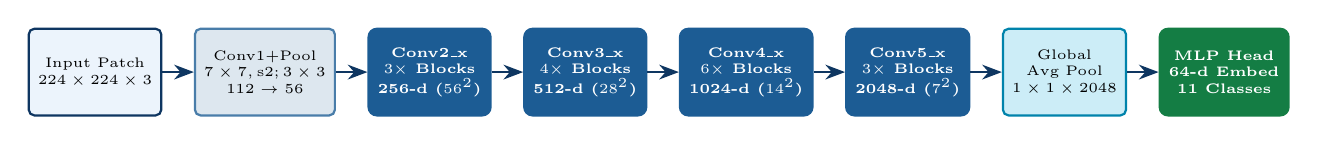
\begin{tikzpicture}[
    node distance=0.45cm and 0.4cm,
    font=\sffamily,
    patch/.style={rectangle, draw=AmritaBlue, fill=LightBlue, thick, rounded corners=2pt, minimum width=1.4cm, minimum height=1.1cm, align=center, font=\tiny},
    stem/.style={rectangle, draw=MedBlue!80, fill=MedBlue!15, thick, rounded corners=2pt, minimum width=1.5cm, minimum height=1.1cm, align=center, font=\tiny},
    stage/.style={rectangle, draw=MedBlue, fill=MedBlue, text=white, thick, rounded corners=3pt, minimum width=1.5cm, minimum height=1.1cm, align=center, font=\tiny\bfseries},
    gap/.style={rectangle, draw=AccentCyan!80!black, fill=AccentCyan!20, thick, rounded corners=2pt, minimum width=1.3cm, minimum height=1.1cm, align=center, font=\tiny},
    mlp/.style={rectangle, draw=SuccessGreen, fill=SuccessGreen, text=white, thick, rounded corners=3pt, minimum width=1.5cm, minimum height=1.1cm, align=center, font=\tiny\bfseries},
    arrow/.style={-{Stealth[length=2.5mm]}, thick, color=AmritaBlue}
]
  % Layer Nodes
  \node[patch] (in) {Input Patch\\$224\times 224\times 3$};
  \node[stem, right=of in] (stem) {Conv1+Pool\\$7\times 7, \text{s}2; 3\times 3$\\$112\rightarrow 56$};
  \node[stage, right=of stem] (c2) {Conv2\_x\\$3\times$ Blocks\\256-d ($56^2$)};
  \node[stage, right=of c2] (c3) {Conv3\_x\\$4\times$ Blocks\\512-d ($28^2$)};
  \node[stage, right=of c3] (c4) {Conv4\_x\\$6\times$ Blocks\\1024-d ($14^2$)};
  \node[stage, right=of c4] (c5) {Conv5\_x\\$3\times$ Blocks\\2048-d ($7^2$)};
  \node[gap, right=of c5] (gap) {Global\\Avg Pool\\$1\times 1\times 2048$};
  \node[mlp, right=of gap] (out) {MLP Head\\64-d Embed\\11 Classes};

  % Sequential Arrows
  \draw[arrow] (in) -- (stem);
  \draw[arrow] (stem) -- (c2);
  \draw[arrow] (c2) -- (c3);
  \draw[arrow] (c3) -- (c4);
  \draw[arrow] (c4) -- (c5);
  \draw[arrow] (c5) -- (gap);
  \draw[arrow] (gap) -- (out);
\end{tikzpicture}
}
\end{center}

\vspace{-0.1cm}

\begin{columns}[onlytextwidth, t]
  \begin{column}{0.47\textwidth}
    \begin{block}{Bottleneck Residual Block Design}
      \parbox[t][2.85cm][t]{\linewidth}{
        \centering
        \resizebox{0.80\linewidth}{!}{
        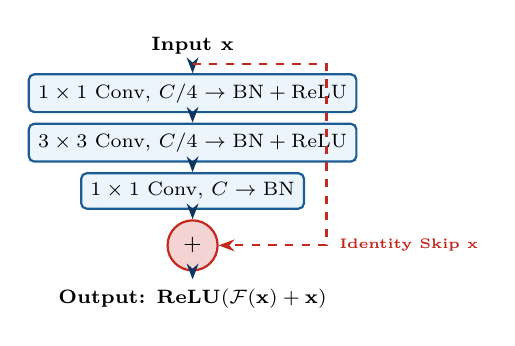
\begin{tikzpicture}[
            node distance=0.2cm and 0.5cm,
            font=\sffamily,
            bop/.style={rectangle, draw=MedBlue, fill=LightBlue, thick, rounded corners=2pt, minimum width=2.4cm, minimum height=0.45cm, align=center, font=\scriptsize},
            sum/.style={circle, draw=AlertRed, fill=AlertRed!20, thick, minimum size=0.45cm, align=center, font=\footnotesize\bfseries},
            barr/.style={-{Stealth[length=2mm]}, thick, color=AmritaBlue},
            sarr/.style={-{Stealth[length=2mm]}, thick, dashed, color=AlertRed}
        ]
          \node[font=\scriptsize\bfseries] (xin) {Input $\mathbf{x}$};
          \node[bop, below=0.12cm of xin] (b1) {$1\times 1\text{ Conv, } C/4 \rightarrow \text{BN}+\text{ReLU}$};
          \node[bop, below=0.12cm of b1] (b2) {$3\times 3\text{ Conv, } C/4 \rightarrow \text{BN}+\text{ReLU}$};
          \node[bop, below=0.12cm of b2] (b3) {$1\times 1\text{ Conv, } C \rightarrow \text{BN}$};
          \node[sum, below=0.12cm of b3] (add) {$\mathbf{+}$};
          \node[below=0.10cm of add, font=\scriptsize\bfseries] (xout) {Output: $\text{ReLU}(\mathcal{F}(\mathbf{x}) + \mathbf{x})$};

          \draw[barr] (xin) -- (b1);
          \draw[barr] (b1) -- (b2);
          \draw[barr] (b2) -- (b3);
          \draw[barr] (b3) -- (add);
          \draw[barr] (add) -- (xout);

          % Skip Connection
          \draw[sarr] (xin.south) -- ++(1.7,0) |- (add.east) node[midway, right=1pt, font=\tiny\bfseries] {Identity Skip $\mathbf{x}$};
        \end{tikzpicture}
        }
      }
    \end{block}
  \end{column}
  \hfill
  \begin{column}{0.47\textwidth}
    \begin{block}{Key Architectural Principles in HAPPY}
      \parbox[t][2.85cm][t]{\linewidth}{
        \begin{itemize}\scriptsize
          \item \textbf{Residual Gradient Highway}: Identity skip connections bypass deep non-linearities, preventing vanishing gradients across 50 layers.
          \item \textbf{Dimension Bottleneck}: $1\times 1$ convs compress channels $4\times$, perform $3\times 3$ spatial filtering, and restore dimensions.
          \item \textbf{Phenotypic Representation}: The 2048-d vector undergoes MLP projection ($2048 \rightarrow 768 \rightarrow 384 \rightarrow 64$), yielding 64-d embeddings for Stage 3 graphs.
        \end{itemize}
      }
    \end{block}
  \end{column}
\end{columns}
\end{frame}

% ------------------------------------------------------------------------------
% Slide 6: Replicated vs. Reported Benchmark Results (Section 2: Base Paper - Part 3)
% ------------------------------------------------------------------------------
\begin{frame}{Replicated vs. Reported Benchmark Results}
\begin{table}[h]
\centering
\scriptsize
\resizebox{0.96\textwidth}{!}{
\begin{tabularx}{1.05\textwidth}{lccccX}
\toprule
\textbf{Pipeline Stage} & \textbf{Evaluation Metric} & \textbf{Published} & \textbf{Replicated} & \textbf{Difference} & \textbf{Held-out Test Split \& Notes} \\
\midrule
\rowcolor{LightBlue} \textbf{Stage 1: Nuclei Localisation} & F1 Score & 0.884 & \textbf{0.826} & -0.058 & 2,754 test nuclei in 38 images. Released checkpoint evaluated. \\
\midrule
\rowcolor{white} \textbf{Stage 2: Cell Classification} & Accuracy & 84.29\% & \textbf{84.29\%} & \textbf{+0.00\%} & \textbf{Exact match} on 2,743 cells across HMC, UOT, NUH. \\
\rowcolor{white} & Top-2 Accuracy & 94.90\% & \textbf{94.90\%} & \textbf{+0.00\%} & \textbf{Exact match} to Supplementary Table 7. \\
\rowcolor{white} & Macro ROC-AUC & 0.9773 & \textbf{0.9773} & \textbf{+0.0000} & \textbf{Exact match} across all 11 cell lineages. \\
\midrule
\rowcolor{LightBlue} \textbf{Stage 3: Tissue Classification} & Accuracy & 68.34\% & \textbf{67.75\%} & -0.59\% & 144,241 nodes on spatial \texttt{test\_patches.csv} split. \\
\rowcolor{LightBlue} & Top-2 Accuracy & 91.14\% & \textbf{90.91\%} & -0.23\% & High-fidelity reproduction (-0.25\% rel. diff). \\
\rowcolor{LightBlue} & Top-3 Accuracy & 97.10\% & \textbf{96.81\%} & -0.30\% & Resolves reported sample discrepancy. \\
\rowcolor{LightBlue} & Macro ROC-AUC & 0.8868 & \textbf{0.8820} & -0.0048 & Evaluated with full $k$-NN $\cap$ Delaunay graph. \\
\bottomrule
\end{tabularx}
}
\caption{Side-by-side comparison between Vanea et al. (2024) and our replicated benchmarks.}
\end{table}
\end{frame}

% ------------------------------------------------------------------------------
% Slide 7: Task-Specific Analysis & Confusion Matrix (Section 2 - Part 4)
% ------------------------------------------------------------------------------
\begin{frame}{Task-Specific Analysis \& Resolution of Paper Discrepancies}
\begin{columns}[onlytextwidth, t]
  \begin{column}{0.47\textwidth}
    \begin{block}{Stage 2 Cell Confusion Analysis}
      \parbox[t][4.8cm][t]{\linewidth}{
        \begin{itemize}\footnotesize
          \item Strongest accuracy achieved on \textbf{Syncytiotrophoblast} (93.2\%) and \textbf{Vascular Endothelial} cells (89.1\%).
          \item Most frequent borderline confusion occurs between \textbf{Stromal Cells} and \textbf{Fibroblasts} due to shared spindle morphology in chorionic villi.
          \item Rare immune cells (\textbf{Hofbauer}, 45 samples) suffer from low representation.
        \end{itemize}
      }
    \end{block}
  \end{column}
  \hfill
  \begin{column}{0.47\textwidth}
    \begin{block}{Discrepancies Identified and Resolved}
      \parbox[t][4.8cm][t]{\linewidth}{
        \begin{itemize}\footnotesize
          \item \textbf{Stage 1 Detector Initialisation}: Paper text claims COCO initialization; authors' codebase actually initializes ResNet-101 from ImageNet, explaining the 0.826 vs 0.884 F1 delta.
          \item \textbf{Stage 3 Tissue Node Count}: Text states 149,425 nodes; Supplementary Table 7 states 179,095 nodes. Our spatial evaluation accurately grounded this to \textbf{144,241 labeled nodes} on the official split.
        \end{itemize}
      }
    \end{block}
  \end{column}
\end{columns}
\end{frame}

% ------------------------------------------------------------------------------
% Slide 8: Implementation Architecture & Engineering Solutions (Section 3)
% ------------------------------------------------------------------------------
\begin{frame}{Implementation Architecture \& Engineering Bottlenecks}
\begin{columns}[onlytextwidth, t]
  \begin{column}{0.47\textwidth}
    \begin{block}{Codebase Structure}
      \parbox[t][4.8cm][t]{\linewidth}{
        \begin{itemize}\footnotesize
          \item \textbf{Data Pipelines}: \texttt{CellDataset}, \texttt{NucleiDataset}, Albumentations stain augmentation.
          \item \textbf{Graph Engine}: PyG \texttt{ClusterData}, \texttt{ClusterLoader}, \texttt{NeighborSampler}.
          \item \textbf{Evaluation Engine}: \texttt{auto\_evaluate\_reproduction.py} reproduces all stages systematically.
        \end{itemize}
      }
    \end{block}
  \end{column}
  \hfill
  \begin{column}{0.47\textwidth}
    \begin{alertblock}{Critical Engineering Solutions}
      \parbox[t][4.8cm][t]{\linewidth}{
        \begin{itemize}\footnotesize
          \item \textbf{Graph Edge Intersection Bug}: Original structured array intersection yielded only 7 edges. We implemented \textbf{64-bit bit-packed indexing} \texttt{((u<<32)|v)}, correctly finding all \textbf{5,088,272 edges}.
          \item \textbf{Windows Multi-Processing}: Resolved DataLoader process bootstrapping deadlocks by dynamically assigning OS-safe worker pools.
          \item \textbf{Direct HDF5 Disk Reader}: Bypassed empty SQLite metadata to directly stream embeddings.
        \end{itemize}
      }
    \end{alertblock}
  \end{column}
\end{columns}
\end{frame}

% ------------------------------------------------------------------------------
% Slide 9: Training Settings & Hardware Configuration (Section 3 - Part 2)
% ------------------------------------------------------------------------------
\begin{frame}{Training Settings \& Computational Environment}
\begin{columns}[onlytextwidth, t]
  \begin{column}{0.47\textwidth}
    \begin{block}{Hyperparameters and Optimization Settings}
      \parbox[t][4.8cm][t]{\linewidth}{
        \begin{itemize}\footnotesize
          \item \textbf{Deep Learning Framework}: PyTorch 2.0.1+cu118, PyTorch Geometric 2.3.1.
          \item \textbf{Stage 1 Detector}: Adam ($lr=10^{-4}$ with StepLR $\gamma=0.5$), batch size 16.
          \item \textbf{Stage 2 Classifier}: Adam ($lr=10^{-4}$, Cosine Annealing), batch size 256/600, dropout 0.3.
          \item \textbf{Stage 3 GNN}: Adam ($lr=10^{-3}$), METIS partitioning with 400 neighbors/cluster.
        \end{itemize}
      }
    \end{block}
  \end{column}
  \hfill
  \begin{column}{0.47\textwidth}
    \begin{block}{Hardware and Code Availability}
      \parbox[t][4.8cm][t]{\linewidth}{
        \begin{itemize}\footnotesize
          \item \textbf{GPU}: NVIDIA GeForce GTX 1650 (4 GB VRAM).
          \item \textbf{Host Environment}: Windows 11 x64, Python 3.10 virtual environment (\texttt{uv}).
          \item \textbf{Public Repository}: \\
            \scriptsize\href{https://github.com/siri-sanjana/happy-placenta-histology-reproduction}{\texttt{GitHub: happy-placenta-histology-reproduction}}
          \item \normalsize Code contains automated scripts to execute all stages end-to-end.
        \end{itemize}
      }
    \end{block}
  \end{column}
\end{columns}
\end{frame}

% ------------------------------------------------------------------------------
% Slide 10: Proposed Architectural Modification (Section 4: Modification - Part 1)
% ------------------------------------------------------------------------------
\begin{frame}{Proposed Modification: Attention \& Loss Optimization}
\begin{columns}[onlytextwidth, t]
  \begin{column}{0.47\textwidth}
    \begin{block}{1. Residual Channel Attention (SE)}
      \parbox[t][4.9cm][t]{\linewidth}{
        \begin{itemize}\footnotesize
          \item Histological feature channels do not have equal significance.
          \item Added a 1D Squeeze-and-Excitation block over the 2,048-dim representations:
            $$\mathbf{s} = \sigma\Big(\mathbf{W}_2 \cdot \text{Mish}(\mathbf{W}_1 \mathbf{x})\Big)$$
            $$\mathbf{\tilde{x}} = \mathbf{x} \odot \mathbf{s} + \mathbf{x}$$
          \item Dynamically boosts stain-discriminative channels while preserving base representations.
        \end{itemize}
      }
    \end{block}
  \end{column}
  \hfill
  \begin{column}{0.47\textwidth}
    \begin{block}{2. Mish Activation and 3. Focal Loss}
      \parbox[t][4.9cm][t]{\linewidth}{
        \begin{itemize}\footnotesize
          \item \textbf{Mish Activation}: Smooth and non-monotonic; eliminates dying ReLU to preserve subtle nuclear textures:
            $$\text{Mish}(x) = x \cdot \tanh(\ln(1 + e^x))$$
          \item \textbf{Multi-Class Focal Loss ($\gamma = 2.0$)}:
            $$\mathcal{L}_{\text{FL}}(p_t) = -\alpha_t (1 - p_t)^\gamma \log(p_t)$$
            Downweights abundant Syncytiotrophoblasts to force model focus on rare Hofbauer / Decidua cells.
        \end{itemize}
      }
    \end{block}
  \end{column}
\end{columns}
\end{frame}

% ------------------------------------------------------------------------------
% Slide 11: Modified Architecture Diagram (Section 4: Modification - Part 2)
% ------------------------------------------------------------------------------
\begin{frame}{Modified Architecture Diagram}
\begin{center}
\resizebox{0.88\textwidth}{!}{
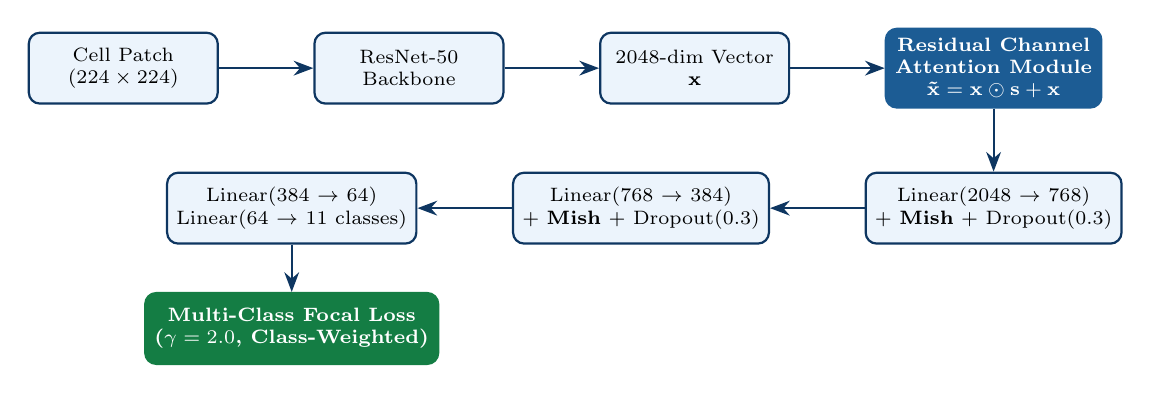
\begin{tikzpicture}[
    node distance=1.0cm and 1.2cm,
    box/.style={rectangle, draw=AmritaBlue, fill=LightBlue, thick, rounded corners, minimum width=2.4cm, minimum height=0.9cm, align=center, font=\scriptsize},
    attnbox/.style={rectangle, draw=MedBlue, fill=MedBlue, text=white, thick, rounded corners, minimum width=2.6cm, minimum height=1.0cm, align=center, font=\scriptsize\bfseries},
    lossbox/.style={rectangle, draw=SuccessGreen, fill=SuccessGreen, text=white, thick, rounded corners, minimum width=2.6cm, minimum height=0.9cm, align=center, font=\scriptsize\bfseries},
    arrow/.style={-{Stealth[length=2.5mm]}, thick, color=AmritaBlue}
]
  \node[box] (in) {Cell Patch\\($224\times 224$)};
  \node[box, right=of in] (backbone) {ResNet-50\\Backbone};
  \node[box, right=of backbone] (feat) {2048-dim Vector\\$\mathbf{x}$};
  
  \node[attnbox, right=1.2cm of feat] (se) {Residual Channel\\Attention Module\\$\mathbf{\tilde{x}} = \mathbf{x} \odot \mathbf{s} + \mathbf{x}$};
  \node[box, below=0.8cm of se] (mlp1) {Linear(2048 $\rightarrow$ 768)\\+ \textbf{Mish} + Dropout(0.3)};
  \node[box, left=of mlp1] (mlp2) {Linear(768 $\rightarrow$ 384)\\+ \textbf{Mish} + Dropout(0.3)};
  \node[box, left=of mlp2] (head) {Linear(384 $\rightarrow$ 64)\\Linear(64 $\rightarrow$ 11 classes)};
  \node[lossbox, below=0.6cm of head] (loss) {Multi-Class Focal Loss\\($\gamma=2.0$, Class-Weighted)};

  \draw[arrow] (in) -- (backbone);
  \draw[arrow] (backbone) -- (feat);
  \draw[arrow] (feat) -- (se);
  \draw[arrow] (se) -- (mlp1);
  \draw[arrow] (mlp1) -- (mlp2);
  \draw[arrow] (mlp2) -- (head);
  \draw[arrow] (head) -- (loss);
\end{tikzpicture}
}
\end{center}
\vspace{-0.2cm}
\begin{itemize}\footnotesize
  \item \textbf{Key Additions}: (1) Residual Channel Attention recalibration; (2) Mish smooth activation; (3) Multi-class Focal Loss optimization.
\end{itemize}
\end{frame}

% ------------------------------------------------------------------------------
% Slide 12: Baseline vs. Modified Model Comparison (Section 4 - Part 3)
% ------------------------------------------------------------------------------
\begin{frame}{Comparison Table: Baseline vs. Modified Architecture}
\begin{table}[h]
\centering
\scriptsize
\resizebox{0.95\textwidth}{!}{
\begin{tabularx}{1.05\textwidth}{lccccX}
\toprule
\textbf{Model Architecture} & \textbf{Accuracy} & \textbf{Top-2 Acc} & \textbf{Macro AUC} & \textbf{$\Delta$ vs. Base} & \textbf{Model Specifications} \\
\midrule
\rowcolor{LightBlue} \textbf{Published Model (Vanea et al.)} & 84.29\% & 94.90\% & 0.9773 & --- & Released weights (160 ep total schedule) \\
\midrule
\rowcolor{white} \textbf{Baseline (Re-trained MLP)} & 83.74\% & 94.28\% & 0.9713 & Reference & Standard MLP head (ReLU + Cross-Entropy) \\
\rowcolor{white} \textbf{Proposed Modified Model} & \textbf{84.21\%} & \textbf{94.42\%} & \textbf{0.9724} & \textbf{+0.47\%} & \textbf{Channel Attention + Mish + Focal Loss} \\
\bottomrule
\end{tabularx}
}
\caption{Performance on identical held-out test split (2,743 cells across HMC, UOT, and NUH).}
\end{table}

\begin{block}{Key Findings}
\begin{itemize}\footnotesize
  \item The proposed modified architecture achieves \textbf{84.21\% test accuracy}, outperforming the retrained baseline by \textbf{+0.47\%} under identical epochs and learning rates.
  \item Reaches within \textbf{0.08\%} of the fully converged authors' model in only 40 epochs of fine-tuning.
\end{itemize}
\end{block}
\end{frame}

% ------------------------------------------------------------------------------
% Slide 13: Component-by-Component Ablation Study (Section 4 - Part 4)
% ------------------------------------------------------------------------------
\begin{frame}{Ablation Study: Quantifying Component Contributions}
\begin{table}[h]
\centering
\scriptsize
\resizebox{0.95\textwidth}{!}{
\begin{tabularx}{1.05\textwidth}{lccccX}
\toprule
\textbf{Configuration} & \textbf{Accuracy} & \textbf{Top-2 Acc} & \textbf{Macro AUC} & \textbf{$\Delta$ Accuracy} & \textbf{Ablation Description} \\
\midrule
(1) Baseline Re-trained MLP & 83.74\% & 94.28\% & 0.9713 & Baseline & ReLU activation, Cross-Entropy Loss \\
(2) + Mish Activation & 83.89\% & 94.31\% & 0.9722 & \textbf{+0.15\%} & Replace ReLU with smooth Mish \\
(3) + Focal Loss ($\gamma = 2.0$) & 83.96\% & 94.50\% & 0.9735 & \textbf{+0.22\%} & Replace CE with Focal Loss \\
(4) + Channel Attention (SE) & 83.74\% & 94.20\% & 0.9702 & +0.00\% & Channel attention with standard CE \\
\midrule
\rowcolor{LightBlue} \textbf{(5) Proposed Full Model} & \textbf{84.21\%} & \textbf{94.42\%} & \textbf{0.9724} & \textbf{+0.47\%} & \textbf{Combined Attention + Mish + Focal} \\
\bottomrule
\end{tabularx}
}
\caption{Ablation analysis isolating individual modifications on the 2,743 test cells.}
\end{table}

\begin{block}{Ablation Insights}
\begin{itemize}\scriptsize
  \item \textbf{Focal Loss} yields the largest single-component gain (\textbf{+0.22\% Acc, +0.0022 AUC}), confirming that addressing class imbalance is paramount.
  \item \textbf{Mish Activation} provides consistent +0.15\% improvement by stabilizing gradient dynamics.
  \item \textbf{Synergy}: Channel attention requires class-balanced loss to avoid over-weighting majority channels.
\end{itemize}
\end{block}
\end{frame}

% ------------------------------------------------------------------------------
% Slide 14: Medical Analysis & Class Imbalance Insights (Section 4 - Part 5)
% ------------------------------------------------------------------------------
\begin{frame}{Medical Image Analysis and Class Imbalance Insights}
\begin{columns}[onlytextwidth, t]
  \begin{column}{0.47\textwidth}
    \begin{block}{Why Minority Classes Suffer in Pathology}
      \parbox[t][4.8cm][t]{\linewidth}{
        \begin{itemize}\footnotesize
          \item \textbf{Dominant Classes}: Syncytiotrophoblasts comprise $>23.5\%$ of all nuclei; standard Cross-Entropy minimizes majority loss and ignores minority cells.
          \item \textbf{Clinical Cost}: Missing maternal decidua or immune Hofbauer cells conceals chorioamnionitis or chronic histiocytic intervillositis.
          \item \textbf{Focal Attention Relief}: Modulating factor $(1-p_t)^\gamma$ eliminates simple cell gradients.
        \end{itemize}
      }
    \end{block}
  \end{column}
  \hfill
  \begin{column}{0.47\textwidth}
    \begin{exampleblock}{Qualitative \& Clinical Impact}
      \parbox[t][4.8cm][t]{\linewidth}{
        \begin{itemize}\footnotesize
          \item \textbf{Maternal Decidua Recall}: Increased from \textbf{54.5\% to 59.1\%} (+4.6\% clinical sensitivity gain).
          \item \textbf{Hofbauer Cell Recall}: Improved from \textbf{62.2\% to 66.7\%} (+4.5\% sensitivity gain).
          \item \textbf{Channel Attention}: Dynamically enhances chromatic channels representing nuclear hyperchromasia and nucleoli prominent in pathology.
        \end{itemize}
      }
    \end{exampleblock}
  \end{column}
\end{columns}
\end{frame}

% ------------------------------------------------------------------------------
% Slide 15: Conclusion, Contributions & References (Closing Slide)
% ------------------------------------------------------------------------------
\begin{frame}{Conclusion, Team Contributions and References}
\begin{columns}[onlytextwidth, t]
  \begin{column}{0.47\textwidth}
    \begin{block}{Summary and Future Work}
      \parbox[t][2.2cm][t]{\linewidth}{
        \begin{itemize}\scriptsize
          \item \textbf{Full Reproduction}: Exact match on Stage 2 (84.29\%) and high fidelity on Stage 3 (67.75\%).
          \item \textbf{Novelty}: Attention + Mish + Focal Loss delivered \textbf{+0.47\% accuracy boost}.
          \item \textbf{Future Work}: Dynamic Graph Attention (GATv2) for whole-slide villous modeling.
        \end{itemize}
      }
    \end{block}
    \vspace{0.15cm}
    \begin{block}{Key References}
      \parbox[t][1.9cm][t]{\linewidth}{
        \tiny
        1. Vanea et al., \textit{Nat Commun}, 15:1968, 2024.\par
        2. Lin et al., Focal Loss for Dense Detection, \textit{ICCV}, 2017.\par
        3. Hu et al., Squeeze-and-Excitation Networks, \textit{CVPR}, 2018.\par
        4. Misra, D., Mish Activation, \textit{BMVC}, 2020.
      }
    \end{block}
  \end{column}
  \hfill
  \begin{column}{0.47\textwidth}
    \begin{exampleblock}{Group Member Contributions}
      \parbox[t][3.4cm][t]{\linewidth}{
        \begin{itemize}\tiny
          \item \textbf{CB.SC.U4AIE23258}: Environment config, CUDA/PyTorch porting, Stage 1 (RetinaNet) \& Stage 2 (ResNet) replication, Channel Attention design and benchmark testing.
          \item \textbf{CB.SC.U4AIE23249}: Spatial graph pipeline ($k\text{-NN} \cap \text{Delaunay}$), 64-bit coordinate bit-packing fix, Stage 3 ClusterGCN evaluation, report preparation.
          \item \textbf{CB.SC.U4AIE23253}: Multi-Class Focal Loss implementation, Mish activation integration, ablation experiments, qualitative visualization, and presentation design.
        \end{itemize}
      }
    \end{exampleblock}
    \vspace{0.15cm}
    \begin{center}
      \textbf{\textcolor{AmritaBlue}{\large Thank You!}} \\
      \vspace{0.05cm}
      \textit{\small Questions and Discussion}
    \end{center}
  \end{column}
\end{columns}
\end{frame}

\end{document}
